\documentclass[11pt]{article}

%% MinionPro fonts 
%\usepackage[lf]{MinionPro}
%\usepackage{MnSymbol}
\usepackage{microtype}

%% Margins
\usepackage{geometry}
\geometry{verbose,letterpaper,tmargin=1in,bmargin=1in,lmargin=1in,rmargin=1in}

%% Other packages
\usepackage{amsmath}
\usepackage{amsthm}
\usepackage[shortlabels]{enumitem}
\usepackage{titlesec}
\usepackage{soul}
\usepackage{tikz}
\usepackage{mathtools}
\usepackage{pgfplots}
\usepackage{tikz-3dplot}
\usepackage{algorithmic}
\usepackage[export]{adjustbox}
\usepackage{tcolorbox}

%% Paragraph style settings
\setlength{\parskip}{\medskipamount}
\setlength{\parindent}{0pt}

%% Change itemize bullets
\renewcommand{\labelitemi}{$\bullet$}
\renewcommand{\labelitemii}{$\circ$}
\renewcommand{\labelitemiii}{$\diamond$}
\renewcommand{\labelitemiv}{$\cdot$}

%% Colors
\definecolor{rred}{RGB}{204,0,0}
\definecolor{ggreen}{RGB}{0,145,0}
\definecolor{yyellow}{RGB}{255,185,0}
\definecolor{bblue}{rgb}{0.2,0.2,0.7}
\definecolor{ggray}{RGB}{190,190,190}
\definecolor{ppurple}{RGB}{160,32,240}
\definecolor{oorange}{RGB}{255,165,0}

%% Shrink section fonts
\titleformat*{\section}{\normalsize\bf}
\titleformat*{\subsection}{\normalsize\bf}
\titleformat*{\subsubsection}{\normalsize\it}

% %% Compress the spacing around section titles
\titlespacing*{\section}{0pt}{1.5ex}{0.75ex}
\titlespacing*{\subsection}{0pt}{1ex}{0.5ex}
\titlespacing*{\subsubsection}{0pt}{1ex}{0.5ex}

%% amsthm settings
\theoremstyle{definition}
\newtheorem{problem}{Problem}
\newtheorem{example}{Example}
\newtheorem*{theorem}{Theorem}
\newtheorem*{bigthm}{Big Theorem}
\newtheorem*{biggerthm}{Bigger Theorem}
\newtheorem*{bigcor1}{Big Corollary 1}
\newtheorem*{bigcor2}{Big Corollary 2}

%% tikz settings
\usetikzlibrary{calc}
\usetikzlibrary{patterns}
\usetikzlibrary{decorations}
\usepgfplotslibrary{polar}

%% algorithmic setup
\algsetup{linenodelimiter=}
\renewcommand{\algorithmiccomment}[1]{\quad// #1}
\renewcommand{\algorithmicrequire}{\emph{Input:}}
\renewcommand{\algorithmicensure}{\emph{Output:}}

%% Answer box macros
%% \answerbox{alignment}{width}{height}
\newcommand{\answerbox}[3]{%
  \fbox{%
    \begin{minipage}[#1]{#2}
      \hfill\vspace{#3}
    \end{minipage}
  }
}

%% \answerboxfull{alignment}{height}
\newcommand{\answerboxfull}[2]{%
  \answerbox{#1}{6.38in}{#2} 
}

%% \answerboxone{alignment}{height} -- for first-level bullet
\newcommand{\answerboxone}[2]{%
  \answerbox{#1}{6.0in}{#2} 
}

%% \answerboxtwo{alignment}{height} -- for second-level bullet
\newcommand{\answerboxtwo}[2]{%
  \answerbox{#1}{5.8in}{#2}
}

%% special boxes
\newcommand{\wordbox}{\answerbox{c}{1.2in}{.7cm}}
\newcommand{\catbox}{\answerbox{c}{.5in}{.7cm}}
\newcommand{\letterbox}{\answerbox{c}{.7cm}{.7cm}}

%% Miscellaneous macros
\newcommand{\tstack}[1]{\begin{multlined}[t] #1 \end{multlined}}
\newcommand{\cstack}[1]{\begin{multlined}[c] #1 \end{multlined}}
\newcommand{\ccite}[1]{\only<presentation>{{\scriptsize\color{gray} #1}}\only<article>{{\small [#1]}}}
\newcommand{\grad}{\nabla}
\newcommand{\ra}{\ensuremath{\rightarrow}~}
\newcommand{\maximize}{\text{maximize}}
\newcommand{\minimize}{\text{minimize}}
\newcommand{\subjectto}{\text{subject to}}
\newcommand{\trans}{\mathsf{T}}
\newcommand{\bb}{\mathbf{b}}
\newcommand{\bx}{\mathbf{x}}
\newcommand{\bc}{\mathbf{c}}
\newcommand{\bd}{\mathbf{d}}

%% LP format
%    \begin{align*}
%      \maximize \quad & \mathbf{c}^{\trans} \mathbf{x}\\
%      \subjectto \quad & A \mathbf{x} = \mathbf{b}\\
%                       & \mathbf{x} \ge \mathbf{0}
%    \end{align*}


%% Redefine maketitle
\makeatletter
\renewcommand{\maketitle}{
  \noindent SA405 -- AMP \hfill Rader \#2.42 \\

  \begin{center}\Large{\textbf{\@title}}\end{center}
}
\makeatother

%% ----- Begin document ----- %%
\begin{document}
  
\title{HW3: Network Flows part 2}


\maketitle

\textbf{Problem 1:} Seven types of packages are to be delivered by five trucks. There are three packages of each type, and the capacities of the five trucks are 6, 4, 5, 4, and 3 packages, respectively. Set up a maximum-flow problem that can be used to determine whether the packages can be loaded so that no truck carries two packages of the same type. 

\begin{enumerate}
\item Draw the network diagram for this problem. \emph{Hint: Draw a source and sink node. The source node should be connected to each of the 7 packages and the sink node should be connected to each of the trucks.}
\item Formulate a concrete max flow model that can determine whether the packages can be loaded so that no truck carries two packages of the same type.
\end{enumerate}

\newpage

\textbf{Problem 2:}
(Adapted from Exercise 2.42, p 83) Consider the directed graph, $G = (V, E)$, given below, where each edge $(i,j) \in E$ has associated with it a distance $d_{i,j}$. Assume that node 1 is the source of the network. Our goal is to find the shortest path from node 1 to every other node in the network.

\begin{enumerate}
\item Formulate the concrete model whose solution gives the shortest path from node 1 to every other node in the network.
\item Convert the concrete model from part (1) into a parameterized model.
\end{enumerate}

\begin{center} 
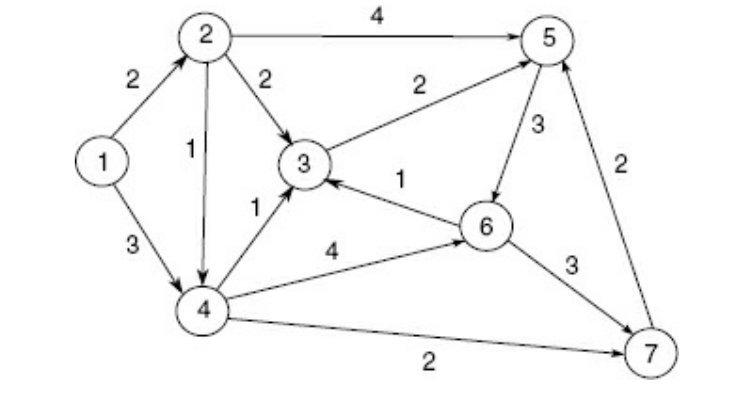
\includegraphics[width=0.9\textwidth]{ShortestPath.png}
\end{center}


\end{document}
